\startchapter{Possibilities for treating experimental data} \label{ch:6}
\section{Description}
The experimental spectra obtained from IR, Raman or SFG techniques have an amplitude scaling factor when comparing to the candidate spectra generated mathematically. This means that between candidates' theoretical spectra and the experimental one, there is an unknown scaling factor. Within one particular spectroscopy technique, this scaling factor is the same for any polarization. Take IR as an example, the scaling factor for the spectrum of $x$ polarization is the same as the one for the spectrum of $z$ polarization. It is necessary to introduce this scaling factor to the LP models. 

\section{Experiments with scaling factor considering each amino acid candidates from $0^{\circ}$ to $80^{\circ}$ on $\theta$}
Since in Chapter \ref{ch:5}, the LP models constructed by Experiment 2 to 7 in Table \ref{tab:5.1} for $\theta$ ranged from $0^{\circ}$ to $80^{\circ}$) are doing well in retrieving the target composition for the mixed amino acids. Therefore, based on these experiments, we would like to know if the same LP models can be applied directly to the real experimental data for the same $\theta$ range.\\

Therefore, the same experiment setting in Table \ref{tab:5.1} are used for the following experiments. The goal is the same, to figure out which spectral information helps to retrieve the target composition for the mixture of six amino acids' candidates. The only difference is that, in each run of the experiment set, an arbitrary scaling factor is generated for IR, Raman and SFG, respectively. Therefore, the target spectra is not only composed by the target composition of all candidates, but also need to multiple by the randomly generated scaling factors of each spectroscopy technique. \\

To start with, we limit the scaling factors to be smaller than 1. \\

After a few runs of the experiment set, it is observed that the returned compositions always contains one extra variable in every experiment. For Experiment 2, 4, 6 and 7, the returned composition contains the right selected candidates. However, the percentage values of the candidates are different from the target composition. The ratio between the returned percentage and the target percentage are the same for the selected candidates. Furthermore, when this ratio adds up the extra variable, it equals $1$. Randomly select one experiment run, then take Experiment 2 as an example. Figure \ref{fig:6.2} displays the target composition generated, only the selected candidates are annotated with assigned percentage. Figure \ref{fig:6.2} displays the return composition of Experiment 2. The selected candidates in the return composition are correct, however, each percentage value is different from the one in the target composition. There are one extra value in Figure \ref{fig:6.2} with value of $0.4$. \\

\begin{figure}[!ht] 
\centering
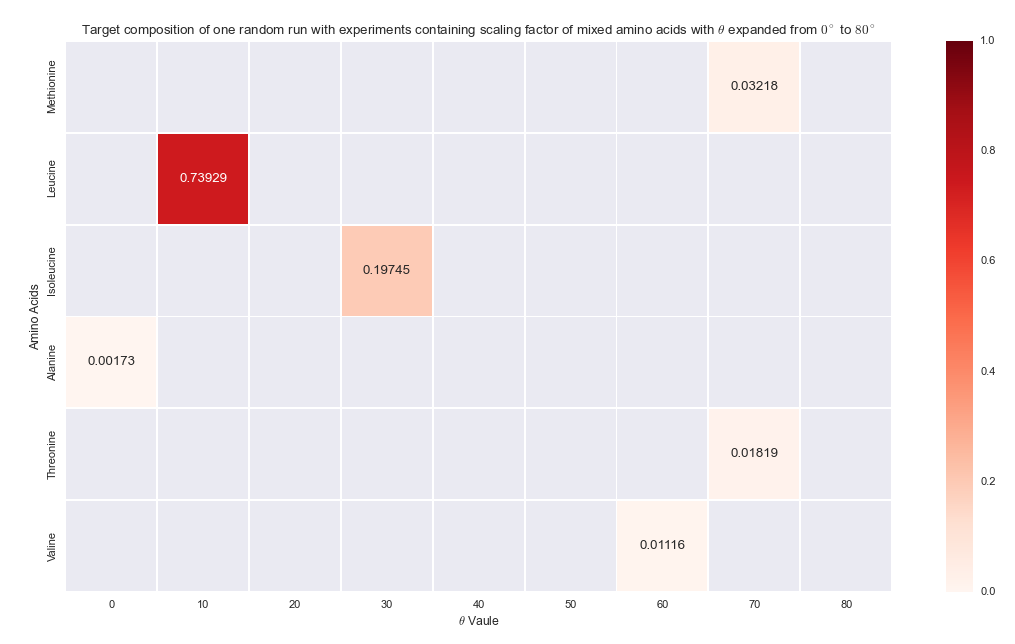
\includegraphics[scale=0.5]{Figures/chapter6_figure_one.png}
\caption{Target composition for one random run of experiment set with scaling foctor for mixed amino acids with $\theta$ expended from $0^{\circ}$ to $80^{\circ}$} \label{fig:6.1}
\end{figure}

\begin{figure}[!ht] 
\centering
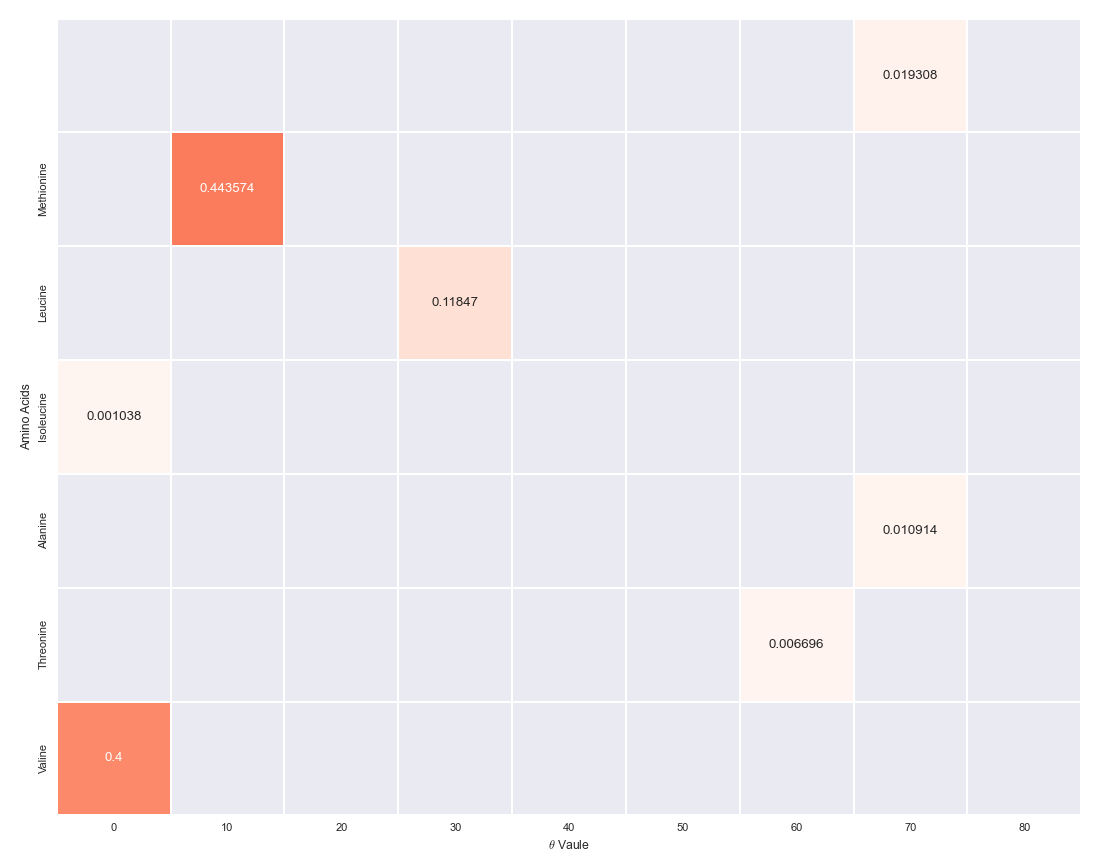
\includegraphics[scale=0.4]{Figures/chapter6_figure_two.png}
\caption{Return composition of Experiment 2 for one random run of experiment set with scaling foctor for mixed amino acids with $\theta$ expended from $0^{\circ}$ to $80^{\circ}$} \label{fig:6.2}
\end{figure}

\begin{figure}[!ht] 
\centering
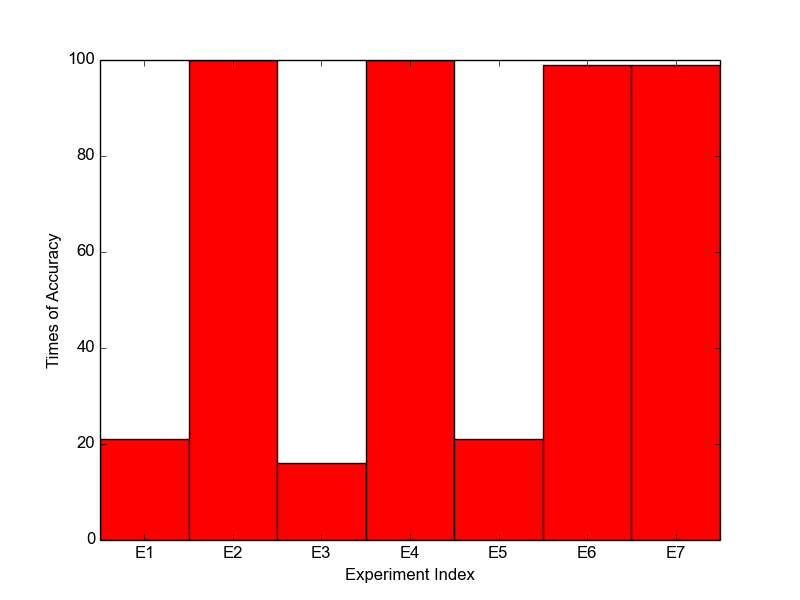
\includegraphics[scale=0.5]{Figures/chapter6_1.png}
\caption{Experiment accuracy analysis for experiments using experimental spectra data that contains scaling factor that is smaller than 1 and candidates with $\theta$ from $0^{\circ}$ to $80^{\circ}$}
\label{fig:6.3}
\end{figure}

Moreover, as Equation \ref{eqn:6.3} shows the ratio between the percentage of the selected candidates in the return composition and the target one is the same for all the amino acids. The value of this ratio is $0.6$. When this ratio is added up with the extra variable (referred as slack variable in LP) $0.4$, the total is $1$. As the scaling factors are pre-generated in the experiment set, the value is known, which is $0.6$. In conclusion, the slack variable (SV) is returned by LP. Then the scaling factor (SF) equals to $1 - SV$. From the scaling factor, the ratio between the return composition and the target one is known. At the end, the target composition can be re-built from the ratio and the return composition. The re-constructed target composition matches to the original one. \\

\begin{eqnarray} \label{eqn:6.3}
\frac{0.019308}{0.03218} = \frac{0.443574}{0.73929} = \frac{0.11847}{0.19745} =\frac{0.001038}{0.00173}  = \frac{0.010914}{0.01819} = \frac{0.006696}{0.01116} = 0.6
\end{eqnarray}

To check whether the above observation is a general case, the experiment set in Table \ref{tab:5.1} is run 100 times with randomly generated scaling factors in each run. Figure \ref{fig:6.3} indicates the experiment result. Figure \ref{fig:6.3} shows that Experiment 2, 4, 6 and 7 almost hit the above observation with $100\%$ frequency. This indicates that even with the scaling factor, Raman spectral information alone is sufficient to study the mixed molecules' coordination distribution at interfaces. The target composition can be re-constructed correctly from the return slack variable and the return composition. Figure \ref{fig:6.3} also illustrates that Experiment 3, the LP model with only SFG spectral information, does not hit the above observation with high frequency. With the scaling factor as the addition, SFG spectral information is not sufficient to obtain the target composition. Even combining IR and SFG spectral information, the constructed LP model cannot help to reconstruct the target composition. \\

\section{Experiments with scaling factor considering each amino acid candidates from $0^{\circ}$ to $180^{\circ}$ on $\theta$}
When each amino acid's candidates are expanded from $0^{\circ}$ to $180^{\circ}$ on $\theta$, the same experiment set is applied 100 times with randomly generated scaling factors in each run. The experiment result from the $100$ run illustrates that none of the experiment in the set meets the above observation with high frequency. \\

However, when further analyze the return compositions of Experiment 2 and 6, there are few other observations need to be noticed. To facilitate the explanation, one random run is picked as an explicit example. Figure \ref{fig:6.4} is the target composition. Figure \ref{fig:6.5} and Figure \ref{fig:6.6} are the return composition of Experiment 2 and Experiment 6. The generated scaling factor for IR, Raman and SFG are $0.863411$, $0.770505$ and $0.239947$. \\

In Figure \ref{fig:6.5}, in the return composition of Experiment 2, the slack variable equals $1-SF = 1-0.770505 = 0.229495$. For each amino acid, the selected candidate in the return composition may not be the exact one as shown in the target composition. However, this selected candidate is always either the correct one, or the correct one's $\theta$ complimentary. Moreover, the ratios between the percentage of each selected candidate in Figure \ref{fig:6.5} and Figure \ref{fig:6.4} is shown in Equation \ref{eqn:6.2}. These ratios all equal to the scaling factor of Raman. \\

In Figure \ref{fig:6.5}, for each amino acid, there are two selected candidates in the return composition. These two selected candidates are the correct one and its $\theta$ complimentary. When the percentages of these two selected candidates are added, it is equalled to the percentage returned for the amino acid in Figure \ref{fig:6.4}. $0.27162 + 0.142619 = 0.414239$. Between these two selected candidates, the correct one's percentage is always bigger than its $\theta$ complimentary. $0.27162 > 0.142619$. In conclusion, Experiment 2 achieves in telling the slack variable, the scaling factor, and the ratio between the returned candidates and the target ones. However, in order to distinguish the exact candidate of each amino acid, the extra information from Experiment 6 is required. Experiment 6 is needed to tell the correct candidate from its complementary on $\theta$. Together with the return information from Experiment 2 and 6, the target composition can be obtained. These observations can be applied to every run of the experiment set.\\


\begin{figure}[!ht] 
\centering
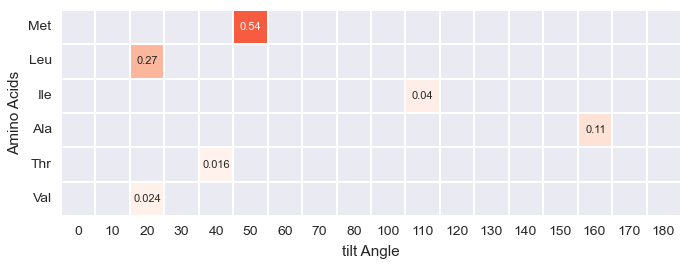
\includegraphics[scale=0.5]{Figures/chapter6_figure_five.png}
\caption{Target composition of  one random run of experiments containing scaling factor and the mixed amino acids' candidates with $\theta$ expended from $0^{\circ}$ to $180^{\circ}$} \label{fig:6.4}
\end{figure}

\begin{figure}[!ht] 
\centering
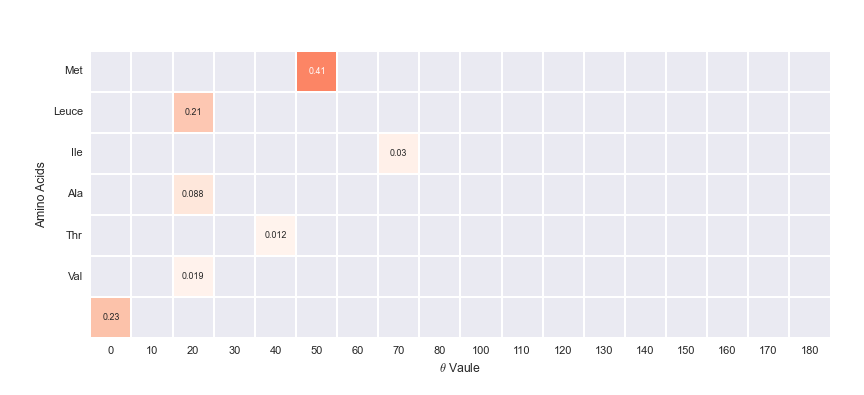
\includegraphics[scale=0.5]{Figures/chapter6_figure_three.png}
\caption{Return composition of Experiment 2 for one random run of experiments containing scaling factor and the mixed amino acids' candidates with $\theta$ expended from $0^{\circ}$ to $180^{\circ}$} \label{fig:6.5}
\end{figure}

\begin{figure}[!ht] 
\centering
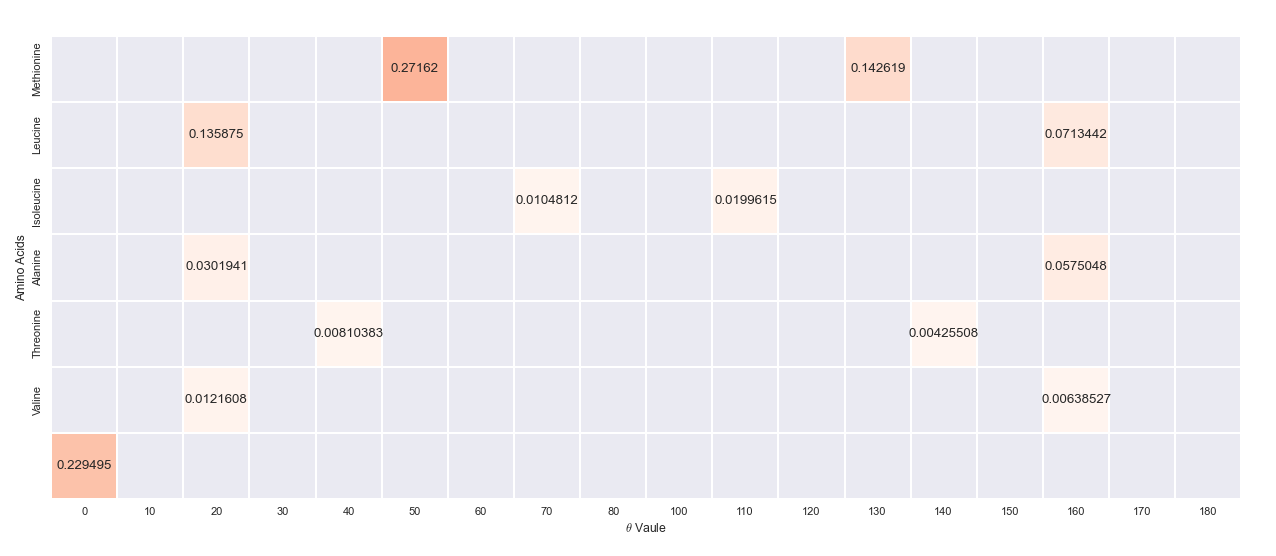
\includegraphics[scale=0.5]{Figures/chapter6_figure_four.png}
\caption{Return composition of Experiment 6 for one random run of experiments containing scaling factor and the mixed amino acids' candidates with $\theta$ expended from $0^{\circ}$ to $180^{\circ}$} \label{fig:6.6}
\end{figure}

\begin{eqnarray} 
\begin{split}
\frac{0.414239}{0.53762} &= \frac{0.20722}{0.26894} = \frac{0.0304427}{0.03951}  =\frac{0.0876989}{0.11382} = \frac{0.0123589}{0.01604} = \frac{0.0185461}{0.02407} = 0.770505
\end{split}\label{eqn:6.2}
\end{eqnarray}

\section{Conclusion}

